Ideally, the score assigned by the model to a decoy should not depend
on its position and orientation.  To allow the model to learn this
invariance, we have randomly sampled the rotational and translational
degrees of freedom of all decoy structures during the training.
%
Figure~\ref{Fig:DecoysScoreDistribution} shows the distributions of
scores for several decoy structures of the same target (T0832),
calculated for 900 rotations and translations sampled uniformly.
While the score of a given structure is not strictly invariant under
rotation and translation, it has a relatively narrow, unimodal
distribution.
%%% GL: I'm saying ``unimodal'' instead of ``Gaussian'' because the
%%% distributions of Figure 6 do not appear to be Gaussian.
%G: Got it
More importantly, the difference between the average scores of two
decoys is usually larger than their variances. To reduce the influence
of the choice of rotation and translation on the final ranking, we
estimate the score of each decoy from the average of 90 scores
calculated for random rotations and translations.

%%% GL: Figure 5 should go in Supporting information. It's showing a
%%% somewhat minor point (about the effect of rotations versus
%%% translations). Figure 6 tells it all.
%G: I moved this figure to the SI

%%% GL: For consistency, can you show use the same reddish color for
%%% this histogram as the one you use in Figure 6? (for
%%% FALCON_EnvFold_TS1). Also, can you use black lines for the
%%% ``rotations'' histogram?
%G: to do conversion from tif to eps using photoshop

%%% GL: I would remove the Gaussian distribution curve. It's somewhat
%%% of an over-interpretation.
%G: to do conversion from tif to eps using photoshop



\begin{figure}[H]
    \centering
    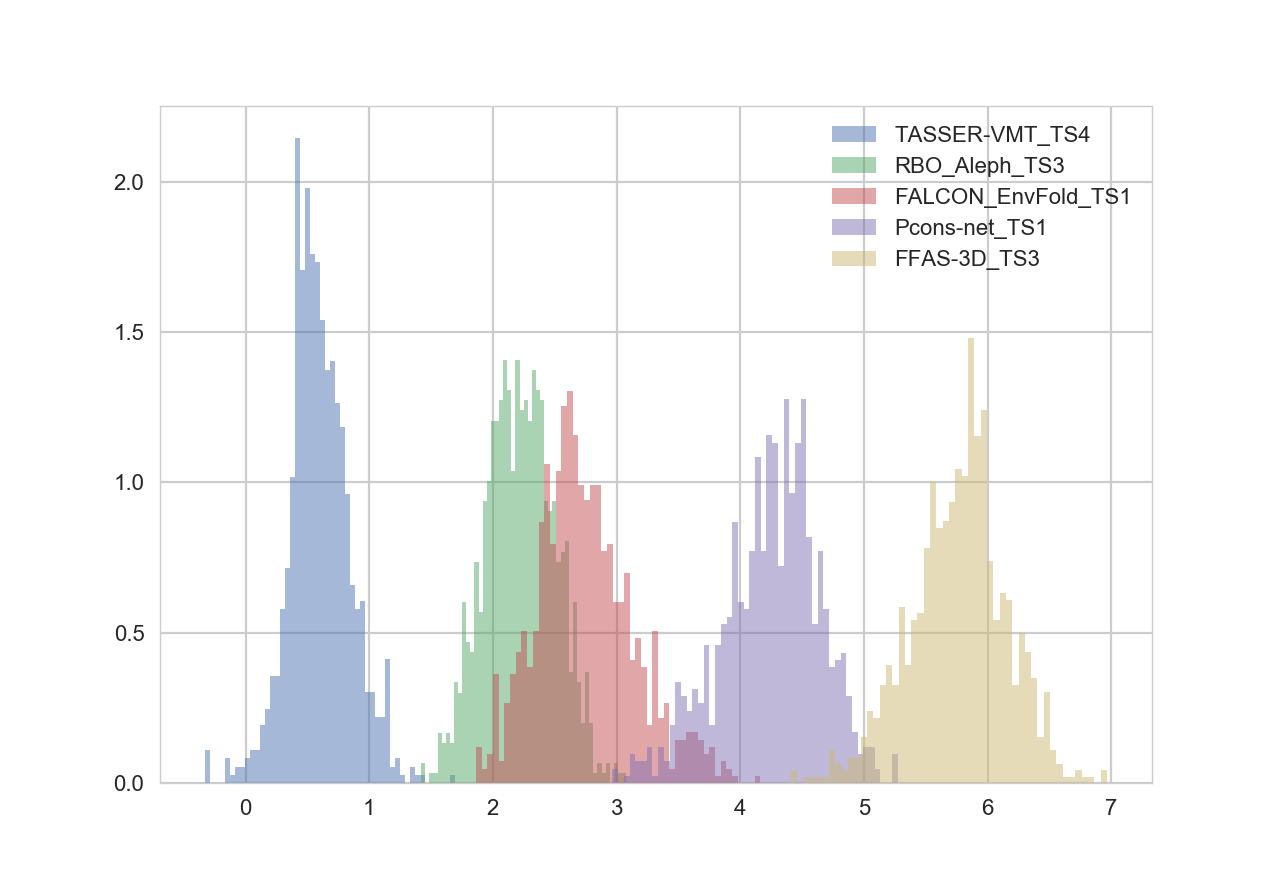
\includegraphics[width=\linewidth]{Fig/decoys_sampling_dist.eps}
%
    \caption{Distributions of the scores of five decoys for target
    T0832 under random translations and rotations. A higher score
    represents a lower quality.}
%
    \label{Fig:DecoysScoreDistribution}
\end{figure}

Table~\ref{Tbl:TestResults} shows a comparison of our model (3DCNN)
with state-of-the-art model quality assessement methods: ProQ2D,
ProQ3D~\cite{uziela2017proq3d}, VoroMQA~\cite{olechnovivc2017voromqa}
and RWPlus~\cite{zhang2010novel}.
ProQ2D uses carefully tuned features based on surface area accessibilities, residue-residue contacts, 
predicted and observed seconday structure, residue conservation and atomic contacts. These features are 
then used as the inputs of deep neural network to predict local and global structure quality. 
ProQ3D employs the same features as ProQ2D as well as Rosetta energy terms based on full-atom and centroid models of the protein. 
This algorithm also uses the features as an input to the deep neural network to predict the 
local and global quality of the candidate structure.
VoroMQA uses knowledge-based potential that depends on the contact surface between two atoms or the solvent. The contact surfaces are calculated 
by representing atoms as spheres with the radii equal to the Van-der-Waals radii of the corresponding atoms and using Voronoi tesselation to obtain 
the contact surface. 
RWPlus is a pairwise knowledge-based potential that uses freely-joined chain model to calculate distance distributions in the reference state.
We chose ProQ2D and ProQ3D as the methods that are derived from the best performing single-model algorithm in CASP11 (ProQ2). The RWPlus 
was selected because it represents previously widespread knowledge-based approach to separate decoys from the corresponding native structures.
VoroMQA was selected, because this approach is rather dissimilar to the common machine-learning techniques and pairwise distance-based scoring potentials.
The other important criterion for selecting these methods is the availability of their source-code or executable. This allowed us to re-evaluate them on 
our CASP11 benchmark, where the decoys side chains were optimized using SCWRL program.

%%% GL: We have to say a few words on each of these methods. What are
%%% they based on? In what sense are they state of the art?
%G: added description of these methods.
%>In what sense are they state of the art?
% This is rather vague question, I wrote why I chose these.

We removed targets T0797, T0798, T0825 from this benchmark, because they were released for multimeric prediction.

\begin{table}[H]
\begin{center}
\begin{tabular}{ c | c | c | c | c }
    MQA method & Loss & Pearson $R$ & Spearmann $\rho$ & Kendall $\tau$ \\ \hline
    \multicolumn{5}{ c }{Stage 1} \\ \hline
    ProQ3D   &0.046 &0.755 &0.673 &0.529 \\
    ProQ2D   &0.064 &0.729 &0.604 &0.468 \\
    \textbf{3DCNN} &0.064 &0.535 &0.425 &0.325 \\    
    VoroMQA  &0.087 &0.637 &0.521 &0.394 \\
    RWplus   &0.122 &0.512 &0.402 &0.303 \\ \hline
    
    \multicolumn{5}{ c }{Stage 2} \\ \hline
    VoroMQA  &0.063 &0.457 &0.449 &0.321 \\ 
    \textbf{3DCNN} &0.064 &0.421 &0.409 &0.288 \\
    ProQ3D   &0.066 &0.452 &0.433 &0.307 \\
    ProQ2D   &0.072 &0.437 &0.422 &0.299 \\
    RWplus   &0.089 &0.206 &0.248 &0.176 \\ \hline

\end{tabular}
%
    \caption{Performance comparison of our method (3DCNN) with other
    state-of-the-art model quality assessment methods on the CASP11
    dataset stages~1 and 2 (see text). The table reports the absolute,
    per-target average values of the correlation coefficients.}
%%% GL: Is it necessary to mention the order in which the averaging is
%%% done? I thought all targets had the same number of decoys.
%G: corrected
    \label{Tbl:TestResults}
\end{center}
\end{table}

